\chapter{Data analysis}
\label{chpt:analysis_appendix}

\section{Photon Streams}
\label{sec:photon_streams_apdx}

In \ac{smFRET} experiments where molecules are freely diffusing in solution, the fluorescence intensity corresponds to the photons counted in the donor and acceptor detectors.
When a fluorophore-labeled molecule diffusing across the confocal volume is excited by a laser, a \enquote{burst} of photons is emitted from the fluorophore (see the time trace in Figure~\ref{fig:smFRET_vs_ensemble}D). 
Thus, a burst is a proxy for a single molecule as it passes through the confocal volume.

Photon streams are determined by the specific detection channel ($D$ or $A$) and the corresponding excitation period. 
In the case of \ac{ALEX}, the excitation periods are either $D$ or $A$, while in \ac{PAX}, the periods are $D$ or $DA$ (the excitation period involving both $D$ and $A$ excitations). 
Each photon is assigned to a particular stream based on its timestamp, $t_i$, and its position within the period, given by $\overline{t_i}$.
The equation for $\overline{t_i}$ considers the possible offset, $t_0$, and employs the modulo arithmetic of the alternation period, $T$:

\begin{equation}
\label{eqn:reduced_t}
\overline{t_i} = (t_i-t_0)mod(T)
\end{equation}

Due to the microsecond response time of the \ac{AOM}, the transition between $D$ to $A$ or $DA$ excitation and vice versa is not instantaneous (see Figure~\ref{fig:alternation_hist}). 
For this reason, photons falling within these transition periods are typically disregarded due to their uncertain origin~\cite{ingargiola_PLOS1_2016}. 
These instances generally constitute a small fraction of the overall photon count ($< 5~\%$).

The histograms representing $\overline{t_i}$ for the donor and acceptor channels serve as practical means to visually delineate these \enquote{excitation periods}\cite{ingargiola_PLOS1_2016} (Figure~\ref{fig:alternation_hist}). 
Table~\ref{tab:ph_streams} indicates the notation used for the photon streams in the two excitation periods.
In the \ac{ALEX} scheme, both donor and acceptor channel histograms show large numbers of photons during donor excitation.
While, during the acceptor excitation period, only the acceptor channel histogram has a substantial photon count (with the donor channel constrained to detector dark count levels).

\begin{figure}
    \centering
    \includegraphics[width=\textwidth]{chapters/figures/alternation_hist.jpg}
    \caption{\label{fig:alternation_hist} 
    $\overline{t_i}$ histograms in ALEX excitation periods.
    The red and green bands indicate the alternation periods in timestamp units.
    The alternation period is $50~\mu$s.
    Timestamps detected in the donor channel during donor excitation ($D_{ex}D_{em}$, i.e. $D$-only excitation) occur during the 2200-3900 period.
    Timestamps detected in the acceptor channel during donor excitation ($D_{ex}A_{em}$, i.e. acceptor fluorescence due to FRET) also occur during the 2200-3900 period.
    Timestamps detected in the acceptor channel during acceptor excitation ($A_{ex}A_{em}$, i.e. $A$-only excitation) occur during the 250-1900 period.
    Timestamps detected in the donor channel during acceptor excitation are ($A_{ex}A_{em}$) are labeled in grey.
    Note that $A_{ex}A_{em}$ photons and photons with timestamps in the transition periods, not highlighted by green and red bands, are discarded in subsequent analyses.
    }
\end{figure}

In the context of \ac{PAX}, both the donor and acceptor channel histograms manifest considerable photon counts throughout both the $D$ and $DA$ excitation periods.

This disparity between the \ac{ALEX} and \ac{PAX} configurations yields distinct definitions for several quantities outlined in subsequent sections.

% \usepackage{tabularray}
\begin{table}
\centering
\caption{\label{tab:ph_streams} Photon streams for \ac{ALEX} and \ac{PAX} alternation schemes. 
The excitation column indicates which laser is on during that period: D indicates 532~nm excitation and A indicates 628~nm excitation. 
Emission is detected in either the $D$ or $A$ channel.}
\begin{tblr}{
  cells = {c},
  cell{5}{4} = {fg=Gray},
  vline{2-4} = {-}{},
  hline{1-2,10} = {-}{},
}
\textbf{Alternation scheme} & \textbf{Excitation} & \textbf{Emission} & \textbf{photon streams} \\
ALEX                        & D                   & D                 & $D_{ex}D_{em}$              \\
                            & D                   & A                 & $D_{ex}A_{em}$              \\
                            & A                   & A                 & $A_{ex}A_{em}$              \\
                            & A                   & D                 & $A_{ex}D_{em}$          \\
PAX                         & D                   & D                 & $D_{ex}D_{em}$              \\
                            & D                   & A                 & $D_{ex}A_{em}$              \\
                            & DA                  & D                 & $DA_{ex}D_{em}$             \\
                            & DA                  & A                 & $DA_{ex}A_{em}$             
\end{tblr}
\end{table}

The raw photon streams, denoted as $F_{X_{ex}Y_{em}}$, correspond to X excitation in the Y emission channel. 
To account for background effects, these streams undergo a background correction involving the subtraction of the averaged background rate, $b_{X_{ex}Y_{em}}$, across the entire period. 
The result is then multiplied by the burst duration, $\Delta T$:

\begin{equation}
\label{eqn:ph_stream}
\overline{F}_{X_{ex}Y_{em}} = F_{X_{ex}Y_{em}} - b_{X_{ex}Y_{em}} \Delta T
\end{equation}

\noindent
where

\begin{equation}
\label{eqn:burst_def}
\Delta T = t_e - t_s
\end{equation}

\noindent
Where $t_s$ is the first timestamp, or the start time, of a burst and $t_e3$, the end time, is the last timestamp of a burst.

In the \ac{PAX} framework, the background-corrected total burst size is given by the summation of the background-corrected photon streams. 
This definition carries a similar meaning in the context of \ac{ALEX}, with the substitution of $DA_{ex}$ by $A_{ex}$:

\begin{equation}
\label{eqn:burst_size}
\overline{F} = \overline{F}_{D_{ex}D_{em}} + \overline{F}_{D_{ex}A_{em}} +\overline{F}_{DA_{ex}D_{em}} + \overline{F}_{DA_{ex}A_{em}}
\end{equation}

\noindent
For FRET efficiency calculations, the total corrected fluorescence during donor excitation, $\overline{F}_D$, is used: 

\begin{equation}
\label{eqn:total_Fd}
\overline{F}_D = \overline{F}_{D_{ex}D_{em}}+\overline{F}_{D_{ex}A_{em}} - Lk - Dir
\end{equation}

\noindent
where $Lk$ is the spectral leakage of the donor signal in the
acceptor channel and $Dir$ is the contribution of direct
excitation of the acceptor dye by the green laser. 
% The correction factors used to compute these quantities are defined in Section~\ref{}.

In PAX, the $\overline{F}_{DA_{ex}D_{em}}$ photon stream 
also contributes information, resulting in improved photon counting statistics
compared to \ac{ALEX}. 
The PAX-specific definition of the corrected fluorescence emission
during donor excitation is given by:

\begin{equation}
\label{eqn:corr_total_Fd}
\overline{F}_{D} = \overline{F}_{D_{ex}D_{em}} + \overline{F}_{DA_{ex}D_{em}} + \alpha^{-1}(\overline{F}_{D_{ex}A_{em}} - Lk - Dir)
\end{equation}

\noindent

Here, $\alpha$ is defined as $\alpha = \left(1 + \frac{\omega_A}{\omega_D}\right)^{-1}$, where $\omega_A$ and $\omega_D$ denote the durations of the $DA_{ex}$ and $D_{ex}$ \ac{PAX} alternation cycles, respectively. 
It's worth noting that these alternation periods typically maintain a duty cycle of $0.5$ and exhibit a ratio of $\omega_A / \omega_D = 1$.

The multiplication by $\alpha^{-1}$ considers the continuous donor excitation, thereby enhancing the $\overline{F}_{D_{ex}A_{em}}$ signal specific to \ac{ALEX}.

%%%%%%%%%%%%%%%%%%%%%%%%%%%%%%%%%%%%%%%%%%%%%%%%%%%%%%%%%%%%%%%%%%%%%%%%%%%

\section{Background rate estimation}
\label{sec:background_rate_apdx}

Background correction, is easily performed using the open-source FRETBursts software~\cite{ingargiola_PLOS1_2016}.

In single-molecule fluorescence experiments, sources contributing to background signal mainly arise from Raleigh and Raman scattering, scattered or out-of-focus fluorescence, sample or buffer impurities, and detector noise (including \ac{DCR}, crosstalk, or afterpulsing effects). 
Effective mitigation of Raleigh and Raman scattering can be achieved with suitable optical filters. 
Although complete elimination of sample impurities is challenging, impurities can be reduced through the use of spectroscopic-grade reagents and buffer filtration.

Precise estimation of the background rate demands careful consideration. Instead of relying on a buffer-only sample as background, the background rate must be calculated for each measurement to account for scattering, out-of-focus fluorescent molecules, and potential fluctuations during measurements. 
One strategy for background rate estimation involves computing the inter-photon delay distribution, $\varphi(\tau)$, for each photon stream. 
The exponential inter-photon delay distribution in a Poisson process can be represented as a weighted summation~\cite{gopich_JCP_2006}:

\begin{equation}
\label{eqn:interphoton_dist}
\varphi\left(\tau\right)\sim \left(1-p_b\right)g\left(\tau\right)+p_bT_be^{-\frac{\tau}{T_b}} 
\end{equation}

\noindent
Here, $g(\tau) \propto \tau^{-3/2}$ represents the distribution of inter-photon delays for a freely diffusing single molecule within a Gaussian excitation volume. 
Additionally, $T_b$ represents the average time between bursts~\cite{gopich_JCP_2006}.

The final term in Eq.~\ref{eqn:interphoton_dist} articulates that the background resulting from out-of-focus molecules can be modeled as a Poisson process with a rate of $b={T_b}^{-1}$, proportional to the concentration. 
Over extended time scales, the exponential term of the weighted sum dominates and serves in computing the background-corrected inter-photon delay distribution.

One approach for estimating the background rate is through the \ac{MLE} for an exponential distribution:

\begin{equation}
\label{eqn:b_inverse}
b^{-1}=\frac{1}{n}\sum_{i=1}^n\tau_i\ =\ <\tau_i>
\end{equation}

\noindent
Where the $\tau_i$ values denote inter-photon delay times. 
Alternate estimators, such as the \ac{MVUE} or the least-squared difference, can also be employed~\cite{ingargiola_PLOS1_2016}. 
However, because the inter-photon delay distribution is exponential and is relevant at extended time scales, the estimation of the background rate is based on the exponential portion of $\varphi(\tau)$. 
The \ac{MLE} for the restricted exponential distribution, where $\tau_i > \tau_{min}$, defines the background rate as:

\begin{equation}
\label{eqn:tau_MLE}
b = \left(\langle \tau_i\rangle_{\tau_i > \tau_{min}} - \tau_{min}\right)^{-1}
\end{equation}

\noindent
Selecting an appropriate value for $\tau_{min}$ involves a trade-off between estimation accuracy and data preservation. 
Using a large value for $\tau_{min}$ leads to a severely truncated dataset, yielding unreliable statistical outcomes. 
Conversely, a small $\tau_{min}$ could introduce bias by disproportionately collecting short inter-photon delay times, linked to single molecules diffusing within the central region of the excitation \ac{PSF}.

Automatic determination of the optimal $\tau_{min}$ is feasible.
A programmatic approach is described in FRETBursts~\cite{ingargiola_PLOS1_2016}.

In numerous single-molecule FRET experiments, the background rate may exhibit variations over time. 
Common causes encompass drift, evaporation, or planned alterations to the sample. 
Due to the fluctuating nature of the background rate, rate estimation must be executed in segments, covering time intervals where the rate remains relatively stable. 
For instance, in the case of rate estimation in a 48-spot setup, a time window of 10 seconds was employed.

In scenarios involving multispot acquisition, these rate estimations must be repeated for each individual spot, as many of the aforementioned parameters vary between spots. 

%%%%%%%%%%%%%%%%%%%%%%%%%%%%%%%%%%%%%%%%%%%%%%%%%%%%%%%%%%%%%%%%%%%%%%%%%%%%
\section{Burst search}
\label{sec:burst_search_apdx}

Following the definition of photon streams and the determination of background rates, the subsequent step in \ac{smFRET} analysis involves a burst search. 
This process entails detecting fluorescent bursts that arise when single molecules pass through the confocal volume, manifesting as spikes above the background signal.

Identification of bursts is performed via a \enquote{sliding window} algorithm, originally introduced by Seidel and colleagues~\cite{eggeling_PNAS_1998, fries_JPCA_1998}. 
Within each sliding window comprised of $m$ consecutive photons, the average photon count rate is computed for one or more photon streams.
It is also possible to perform the burst search over a summation of several photon streams. 
The calculation of the rate, $r_m(t_i)$, is defined as:

\begin{equation}
\label{eqn:local_rate}
r_m(t_i) = \frac{m-2}{t_{i+m-1}-t_i}
\end{equation}

\noindent
where $t_i$ denotes the initial time stamp of the series of $m$ photons utilized for rate computation~\cite{ingargiola_PLOS1_2016}.
A burst is identified when the count rate within that window surpasses a designated threshold rate.
Commonly adopted values for $m$ range from 5 to 15 photons. 
Notably, $m$ also establishes the minimum burst size.

Two approaches can be employed to establish the threshold rate, i) a constant threshold can be defined, or ii) an adaptive moving threshold can be implemented.
Setting a constant threshold for the burst search is common, however this does not account for changes in the background over time.
Opting for an adaptive threshold effectively accommodates potential fluctuations in background levels over time. 
In this case, the threshold is determined proportionally (using a factor denoted as $F$) to the local background rate. 
Generally, typically $F$ ranges between 5 and 10. 
This approach establishes the minimal \ac{SBR} as $(F - 1)$~\cite{michalet_PRSB_2012}.
A comprehensive comparison of the two threshold selection methods is discussed the in the original FRETBursts publication~\cite{ingargiola_PLOS1_2016}.

Typical burst searches are:
\begin{itemize}
\item \ac{APBS}: the burst search is conducted by summing all photon streams together~\cite{nir_JPCB_2006, eggeling_PNAS_1998, fries_JPCA_1998}.
\item \ac{DCBS}: two separate burst searches are performed, one for the donor channel and another for the acceptor channel. 
Only the coincident bursts detected in both searches are retained, and their overlapping segments are kept~\cite{nir_JPCB_2006}.
\end{itemize}

The \ac{DCBS} approach proves valuable for eliminating donor-only and acceptor-only species. 
Moreover, by excluding non-overlapping portions within bursts from the donor and acceptor channels, \ac{DCBS} contributes to reducing the impact of photophysical phenomena like blinking.

There are alternative burst search methods that can be implemented. 
For instance:

\begin{itemize}
    \item The Donor Emission Burst Search ($D_{em}$BS) or Acceptor Emission Burst Search ($A_{em}$BS) involves selecting all photons received in the donor or acceptor channel respectively, without regard for the laser alternation cycle.
    \item The Donor Excitation Burst Search ($D_{ex}$BS) or Acceptor Excitation Burst Search ($A_{ex}$BS) involves selecting all photons received in either channel during the respective $D$ or $A$ laser excitation periods.
\end{itemize}

Both FRETBursts and ALiX offer the flexibility to execute burst searches based on arbitrary logical combinations of photon streams. While numerous options are available, it is often advantageous to begin an analysis by using the \ac{APBS} method, followed by burst selection, a topic explored in Section~\ref{sec:burst_selection_apdx}.

Within this study, burst searches for multispot data were conducted independently for each individual spot. A uniform burst selection threshold was applied to all photons (using \ac{APBS}), and further selections were subsequently applied.

A comprehensive assessment of the impact of various burst search methodologies on burst statistics is detailed in the original FRETBursts publication~\cite{ingargiola_PLOS1_2016}.

%%%%%%%%%%%%%%%%%%%%%%%%%%%%%%%%%%%%%%%%%%%%%%%%%%%%%%%%%%%%%%%%%%%%%%%%%%%%%
\section{Fusing bursts}
\label{sec:fusing_bursts_apdx}

In the analysis of freely diffusing molecules, it's often advantageous to merge, or \enquote{fuse}, bursts that are separated by a time interval less than a specified minimum duration. 
Typically, these bursts correspond to the same molecule entering and exiting the excitation-detection volume successively. 
The fusion of such bursts leads to bursts containing more photons, generally resulting in improved statistical reliability. 
However, this merging process assumes that no changes occur to the molecule during the time between these successive crossings, which does not always hold true~\cite{hoffmann_PCCP_2011}.
For this reason, it is crucial to exercise caution when fusing bursts with a minimum interval that is excessively long, as this can introduce additional noise due to increased background variance.

%%%%%%%%%%%%%%%%%%%%%%%%%%%%%%%%%%%%%%%%%%%%%%%%%%%%%%%%%%%%%%%%%%%%%%%%%%%
\section{Burst selection}
\label{sec:burst_selection_apdx}

Following the burst search process, it is typically necessary to perform a burst selection step as the burst search often returns a considerable number of very small bursts, which can introduce relative variance into the final burst statistics.
Usually, a burst size selection criterion is employed, which excludes bursts with a total size ($\overline{F}$, as defined in Eq.~\ref{eqn:burst_size}) falling below a predetermined threshold, such as $\overline{F} > \overline{F}_{min} = 30$ photons.

In scenarios where different molecular species coexist in the solution, the selection should be performed after the initial burst search and all relevant corrections have been applied. 
This sequence of operations helps minimize bias during the selection process.

Furthermore, additional selections may be carried out for specific analytical objectives. 
For instance, in the context of \ac{PAX}, an extra burst selection based on the $DA_{ex}A_{em}$ photon stream can be employed to retain only FRET species. For detailed computational procedures regarding FRET burst searches and subsequent burst selections, see the \texttt{48-spot-smFRET-PAX-analysis} repository (\href{https://github.com/tritemio/48-spot-smFRET-PAX-analysis}{link})~\cite{ingargiola_JCP_2018}.

%%%%%%%%%%%%%%%%%%%%%%%%%%%%%%%%%%%%%%%%%%%%%%%%%%%%%%%%%%%%%%%%%%%%%%%%%%%%
\section{FRET efficiency,$E$, and stoichiometry ratio, $S$}
\label{sec:ratiometric_E_S_apdx}

The following subsections outline definitions for the uncorrected values of FRET efficiency ($E_{PR}$) and stoichiometry ($S$), and the corresponding corrected values for FRET efficiency ($E$) and stoichiometry ($S_{\gamma\beta}$).
In addition, the differences for the values with respect to the \ac{ALEX} and \ac{PAX} excitation schemes are highlighted.

%%%%%%%%%%%%%%%%%%%%%%%%%%%%%%%%%%%%%%%%%%%%%
\subsection{Proximity ratio, $E_{PR}$}
\label{sec:Epr_apdx}

The ratiometric definition of FRET efficiency varies depending on the specific technique used, primarily relying on the available photon streams. Calculating it accurately can be a complex task, involving considerations such as quantum yield, detection efficiencies, absorption cross-section, and more.

However, in many instances, an approximate value, which does not correct for the these factors, is sufficient for distinguishing between different sub-species and quantifying changes. 
This simplified value is commonly referred to as the \enquote{proximity ratio.}

The proximity ratio, denoted as $E_{PR}$, can be calculated using background-corrected burst sizes, $\overline{F}$, with the following expression:

\begin{equation}
\label{eqn:Epr}
E_{PR}=\frac{\overline{F}_{D_{ex}A_{em}}}{\overline{F}_{D_{ex}A_{em}}+\overline{F}_{D_{ex}D_{em}}}=\frac{\overline{F}_{D_{ex}A_{em}}}{\overline{F}_D}
\end{equation}

\noindent
Here, $\overline{F}_D$ represents the total background-corrected fluorescence during donor excitation. 
The values of $E_{PR}$ typically fall within the range of 0 to 1, where 0 signifies no FRET, and 1 indicates 100\% FRET. 
However, due to imperfect background corrections, values both smaller and larger than this nominal range can also occur.

%%%%%%%%%%%%%%%%%%%%%%%%%%%%%%%%%%%%%%%%%%%%%
\subsection{Uncorrected stoichiometry, $S$}
\label{sec:uncorrected_S_apdx}

The stoichiometry ratio separates different molecular species in single-molecule FRET experiments. It typically ranges from 0 to 1, where specific values have distinct interpretations:

\begin{itemize}
    \item A stoichiometry ratio of $S = 0$ signifies acceptor-only species.
    \item A ratio of $S = 1$ indicates donor-only species.
    \item Doubly-labeled molecules with active dyes, i.e., FRET species, typically exhibit a stoichiometry ratio around $S \approx 1/2$.
\end{itemize}

Similar to the proximity ratio, a fully corrected stoichiometry ratio, denoted as $S_{\gamma\beta}$, can be defined in both \ac{ALEX} and \ac{PAX}~\cite{lee_BPJ_2005,ingargiola_JCP_2018}. 
However, a simpler uncorrected stoichiometry ratio, represented as $S$, can be calculated using the background-corrected burst sizes.

The following expressions allow the calculation of stoichiometry ratios without the need for complex corrections, and reduces error propagation by implementing fewer mathematical steps. 

For \ac{ALEX}, the uncorrected stoichiometry ratio, $S$, is given by:

\begin{equation}
\label{eqn:Salex}
S=\frac{\overline{F}_{D_{ex}D_{em}} + \overline{F}_{D_{ex}A_{em}}}{\overline{F}_{D_{ex}D_{em}} + \overline{F}_{D_{ex}A_{em}}+\overline{F}_{A_{ex}A_{em}}}=\frac{\overline{F}_D}{\overline{F}_D + \overline{F}_{A_{ex}A_{em}}}
\end{equation}

In contrast, \ac{PAX} does not have the $\overline{F}_{A_{ex}A_{em}}$ signal, instead it has a similar quantity, $\overline{F}_{DA_{ex}A_{em}}$.
The \ac{PAX}-specific quantity, $\tilde{F}_{A_{ex}A_{em}}$, can be defined as\cite{ingargiola_JCP_2018}:

\begin{equation}
    \label{eqn:Faa_pax}
    \tilde{F}_{A_{ex}A_{em}} = \overline{F}_{DA_{ex}A_{em}} - \frac{\omega_A}{\omega_D}\overline{F}_{D_{ex}D_{em}}
\end{equation}

\noindent
This definition requires the assumption that excitation intensities do not change between intervals, which typically holds true when the alternation period is sufficiently short.

Using this \ac{PAX}-specific definition, the uncorrected stoichiometry ratio is given by:

\begin{equation}
\label{eqn:Spax}
S = \frac{\overline{F}_D}{\overline{F}_D + \tilde{F}_{A_{ex}A_{em}}}
\end{equation}

\noindent
where $\omega_A$ and $\omega_D$ indicate the durations of the $DA_{ex}$ and $D_{ex}$ \ac{PAX} alternation cycles, respectively.

In the context of \ac{PAX}, an unmodified and uncorrected stoichiometry ratio, denoted as $S_u$, can also be used~\cite{ingargiola_JCP_2018}:

\begin{equation}
\label{eqn:Su}
S_u = \frac{\overline{F}_{D}}{\overline{F}_{D}+\overline{F}_{DA_{ex}A_{em}}}
\end{equation}

\noindent
This expression differs from Eqn.~\ref{eqn:Spax} by omitting subtraction of the $\frac{\omega_A}{\omega_D} \overline{F}_{D_{ex}A_{em}}$ term.

Using $S_u$ over $S$ yields in a lower variance for small bursts. 
Consequently, it can provide improved separation between sub-populations. 
However, it's important to consider that $S_u$ depends on the FRET efficiency, with $S_u$ decreasing as $E$ increases. 
This dependence on FRET efficiency could potentially affect the separation of sub-populations, particularly for species with low FRET efficiency~\cite{ingargiola_JCP_2018}.
Thus, use of $S_u$ should be reserved for situations in which the FRET efficiencies of populations are sufficiently separated.

%%%%%%%%%%%%%%%%%%%%%%%%%%%%%%%%%%%%%%%%%%%%%
\subsection{Corrected FRET efficiency, $E$}
\label{sec:E_apdx}

In a \ac{smFRET} experiment, the $\gamma$ correction factor is used to scale the $D_{ex}D_{em}$ and $D_{ex}A_{em}$ signals. 
It takes into account differences in the quantum yields and photon detection efficiencies of the fluorophores, ensuring that these signals are comparable. 
The definition of $\gamma$ is as follows~\cite{lee_BPJ_2005}:

\begin{equation}
    \label{eqn:gamma}
    \gamma = \frac{\phi_A\eta^{A_{em}}_{A_{det}}}{\phi_D\eta^{D_{em}}_{D_{det}}}
\end{equation}

\noindent
where $\phi_A$ and $\phi_D$ are the quantum yields of the acceptor and donor, and $\eta^{A_{em}}_{A_{det}}$ and $\eta^{D_{em}}_{D_{det}}$ are the detection efficiencies in the acceptor and donor detectors. 

Furthermore, a second correction factor, denoted as $\beta$, is introduced to consider variations in the donor and acceptor excitation rates at their respective excitation wavelengths. 
The definition of $\beta$ is as follows~\cite{lee_BPJ_2005}:

\begin{equation}
    \label{eqn:beta}
    \beta = \frac{I_{A_{ex}}\sigma^{A}_{A_{ex}}}{I_{D_{ex}}\sigma^{D}_{D_{ex}}}
\end{equation}

\noindent
Here, $I_{A_{ex}}$ and $I_{D_{ex}}$ represent the excitation intensities for acceptor and donor, respectively, and $\sigma^{A}_{A_{ex}}$ and $\sigma^{D}_{D_{ex}}$ denote the absorption cross sections of the fluorophores at the wavelength of excitation.

Expanding on $\overline{F}_D$, defined in Eqn.~\ref{eqn:corr_total_Fd}, we introduce the $\gamma$- and background-corrected total fluorescence during donor excitation, $\overline{F}_{D_{\gamma}}$, as~\cite{lee_BPJ_2005, ingargiola_JCP_2018}:

\begin{equation}
    \label{eqn:corr_total_gamma_Fd}
    \overline{F}_{D_{\gamma}} = \gamma\overline{F}_{D_{ex}D_{em}} + F_{FRET}
\end{equation}

\noindent
where $F_{FRET}$ is the leakage and direct-excitation corrected FRET signal ($\overline{F}_{D_{ex}A_{em}}$)~\cite{lee_BPJ_2005, ingargiola_JCP_2018}:

\begin{equation}
    \label{eqn:Ffret}
    F_{FRET} = \overline{F}_{D_{ex}A_{em}} - Lk - Dir
\end{equation}

Given $\overline{F}_{D_{\gamma}}$, we can now define the corrected FRET efficiency, $E$, for both \ac{ALEX} and \ac{PAX} as~\cite{lee_BPJ_2005, ingargiola_JCP_2018}:

\begin{equation}
    \label{eqn:corr_E}
    E = \frac{F_{FRET}}{\overline{F}_{D_{\gamma}}}
\end{equation}

%%%%%%%%%%%%%%%%%%%%%%%%%%%%%%%%%%%%%%%%%%%%%
\subsection{Corrected stoichiometry, $S_{\gamma\beta}$}
\label{sec:S_apdx}

The stoichiometry ratio is different for the \ac{ALEX} and \ac{PAX} excitation schemes. 
In \ac{ALEX} the corrected stoichiometry, $S_{\gamma\beta}$ is defined as~\cite{lee_BPJ_2005, ingargiola_JCP_2018}:

\begin{equation}
    \label{eqn:corr_Salex}
    S_{\gamma\beta} = \frac{\overline{F}_{D_{\gamma}}}{\overline{F}_{D_{\gamma}} + \beta^{-1}F_{A_{ex}A_{em}}}
\end{equation}

The value of $S_{\gamma\beta}$ consistently centers around 0.5 for doubly labeled species, irrespective of FRET efficiency or the donor and acceptor excitation intensities.

The corrected stoichiometry in the context of \ac{PAX} can be defined using the \ac{PAX}-specific quantity, $\tilde{F}_{A_{ex}A_{em}}$ (Eqn.~\ref{eqn:Su})~\cite{ingargiola_JCP_2018}:

\begin{equation}
    \label{eqn:corr_Spax}
    S_{\gamma\beta} = \frac{\overline{F}_{D_{\gamma}}}{\overline{F}_{D_{\gamma}} + \beta^{-1}\tilde{F}_{A_{ex}A_{em}}}
\end{equation}


%%%%%%%%%%%%%%%%%%%%%%%%%%%%%%%%%%%%%%%%%%%%%
\section{$E$, $S$, and $E-S$ Histograms}
\label{sec:E_S_histogram}

The 2-dimensional $E - S$ histogram, more specifically the $E_{PR}-S$ or $E_{PR}-S_u$ histogram, is a valuable visualization tool for separating burst sub-populations based on their stoichiometry and their proximity ratio, in the case of doubly-labeled molecules. 

1-dimensional projections along the $E_{PR}$, $S$, or $S_u$ direction can then be plotted after selecting specific sub-populations of bursts. 
These projections are useful for providing clearer visualizations and quantification of the distributions of $E_{PR}$ and $S$ (or $S_u$).

The quantitative analysis of these histograms remains a subject of ongoing debate, primarily because burst search parameters have a complex impact on these histograms. 
The most rigorous approach involves using the information from each individual burst to compare observed and predicted histograms. 
This is achieved through advanced modeling of various experimental effects inherent in the measurement process, such as shot noise analysis~\cite{nir_JPCB_2006,ingargiola_PLOS1_2016} or photon distribution analysis~\cite{antonik_JPCB_2006}.

For a basic estimation of sub-populations and characteristic values of $E_{PR}$, $S$, or $S_u$ for these populations, fitting the observed histograms with an \textit{ad-hoc} model that provides a qualitative description is suitable.

In this analysis, we employ the following model, which consists of two asymmetric Gaussian distributions connected by a \enquote{bridge.} 
This bridge accounts for a sub-population of bursts attributed to coincident molecule detection or photophysical events such as bleaching and blinking during detection:

\begin{equation}
\label{eqn:two_bridged_peaks_model}
\begin{cases}
f(x) = & A_1 g_1(x) + A_2 g_2(x) + (a + bx) h(x) \\

g_i(x) = & \exp \left(- \frac{(x - x_i)^2}{2 \sigma_i^2} \right), i = 1, 2 \\

\sigma_i = &
\begin{cases}
\sigma_i^- & \text{if}~x < x_i,\\
\sigma_i^+ & \text{if}~x \geq x_i
\end{cases} \\

h(x) = &
\begin{cases}
\left(1-g_1(x) \right) \left(1-g_1(x) \right) & \text{if}~x_1 < x < x_2,\\
0 & \text{otherwise} \\
\end{cases}
\end{cases}
\end{equation}

Excluding the bridging bursts, the integrals beneath the asymmetric Gaussian peaks, $I_i$, offer a reliable estimate of the number of bursts in each sub-population:

\begin{equation}
\label{eqn:AG_peak_integral}
I_i = \sqrt{\pi/2}~A_i \left(\sigma_i^- + \sigma_i^+ \right)/\delta x
\end{equation}

\noindent
where $\delta x$ is the histogram bin width.

%%%%%%%%%%%%%%%%%%%%%%%%%%%%%%%%%%%%%%%%%%%%%%%%%%%%%%%%%%%%%%%%%%%%%%%%%%%

\section{Correction factors}
\label{sec:correction_factors}

To perform accurate \ac{smFRET} analysis, it is necessary to include 
% define \alpha? 
several correction factors denoted as $l$, $d$, $\beta$, and $\gamma$~\cite{lee_BPJ_2005}.
The $\gamma$ and $\beta$ factors have been defined in Section~\ref{sec:ratiometric_E_S_apdx}, and will therefore be omitted from this section.

%%%%%%%%%%%%%%%%%%%%%%%%%%%%%%%%%%%%%%%%%%%%%%
\subsection{Donor leakage factor, $l$}
\label{sec:lk_apdx}

The donor leakage factor, denoted as $l$, is defined as~\cite{lee_BPJ_2005}:

\begin{equation}
\label{eqn:lk}
Lk = l F_{D_{ex}}^{A_{em}}
\end{equation}

\noindent
where $l$ is the donor leakage coefficient, and is defined as~\cite{lee_BPJ_2005}:

\begin{equation}
    \label{eqn:l}
    l = I_{D_{ex}}\sigma^D_{D_{ex}}\phi_D\eta^{D_{em}}_{A_{det}}(1-E) = \frac{\eta^{D_{em}}_{A_{det}}}{\eta^{D_{em}}_{D_{det}}}
\end{equation}

\noindent
Where $I_{D_{ex}}$ is the excitation intensity during the donor excitation period, $\sigma^D_{D_{ex}}$ is the absorption cross section at the donor excitation laser wavelength, $\phi_D$ is the quantum yield of the donor fluorophore, and $\eta^{D_{em}}_{A_{det}}$ is the donor emission detection efficiency in the acceptor channel.

The $l$ correction factor is determined experimentally by analyzing a donor-only (DO) histogram and centering around 0 after correction. 
$l$ can be calculated using the expression:

\begin{equation}
\label{eqn:lk_do}
l = \frac{E_{{PR}_{DO}}}{1-E_{{PR}_{DO}}}
\end{equation}

%%%%%%%%%%%%%%%%%%%%%%%%%%%%%%%%%%%%%%%%%%%%%%%%
\subsection{Direct acceptor excitation factor, $d$}
\label{sec:dir_apdx}

The direct acceptor excitation correction factor, denoted as $d$, is defined as:

\begin{equation}
\label{eqn:dir}
Dir = d F_{A_{ex}}^{A_{em}}
\end{equation}

\noindent
In this equation, $I_{D_{ex}}$ represents the excitation intensity during the donor excitation cycle, $\sigma^A_{D_{ex}}$ is the absorption cross-section of the acceptor dye under donor excitation, $\phi_A$ is the quantum yield of the acceptor fluorophore, and $\eta^{A_{em}}_{A_{det}}$ denotes the detection efficiency of acceptor emission in the acceptor channel.

The $d$ correction factor can be determined experimentally by ensuring that the $S$ histogram of an acceptor-only (AO) sample is centered around 0 after correction. 
If $S_{AO}$ represents the position of that histogram before correction, then:

\begin{equation}
\label{eqn:dir_ao}
d = \frac{S_{AO}}{1-S_{AO}}
\end{equation}

\noindent
In this equation, $S_{AO}$ refers to the background corrected stoichiometry ratio.
Notably, $S_{AO}$ is not corrected for $Lk$ and $Dir$.

%%%%%%%%%%%%%%%%%%%%%%%%%%%%%%%%%%%%%
\subsection{Spot-specific correction factors for \ac{HT-smFRET}}
\label{sec:spot_corrs_apdx}

In previous work on the 48-spot setup~\cite{ingargiola_JCP_2018}, we found that including spot-specific correction factors, like $l$, $d$, and $\gamma$ which theoretically depend on the specific spot under consideration, does not improve the separation of FRET subspecies when the experimental setup is carefully aligned.
Spot-specific corrections are presented in the original 48-spot publication~\cite{ingargiola_JCP_2018}.

%%%%%%%%%%%%%%%%%%%%%%%%%%%%%%%%%%%%%%%%
\section{Burst statistics}
\label{sec:burst_stats_apdx}

Burst analysis is applicable for quantifying not only $E$ and $S$ but also various other parameters related to concentration, diffusivity, brightness, and more. 
The subsequent subsections will provide detailed explanations of burst statistics.

%%%%%%%%%%%%%%%%%%%%%%%%%%%%%%
\subsection{Burst Size}
\label{sec:burst_size_apdx}

Burst size has been previously discussed in the context of burst selection.
It is a useful quantity to histogram as it provides a quick preview of the data. 
Smaller average burst sizes lead to increased variance in any subsequently derived parameters. 
In situations involving multispot data acquisition, this analysis yields a series of burst size histograms, which are often similar or identical, as exemplified in Fig.~\ref{fig:flow_burst_size_48_spots}.

\begin{figure}
\centering
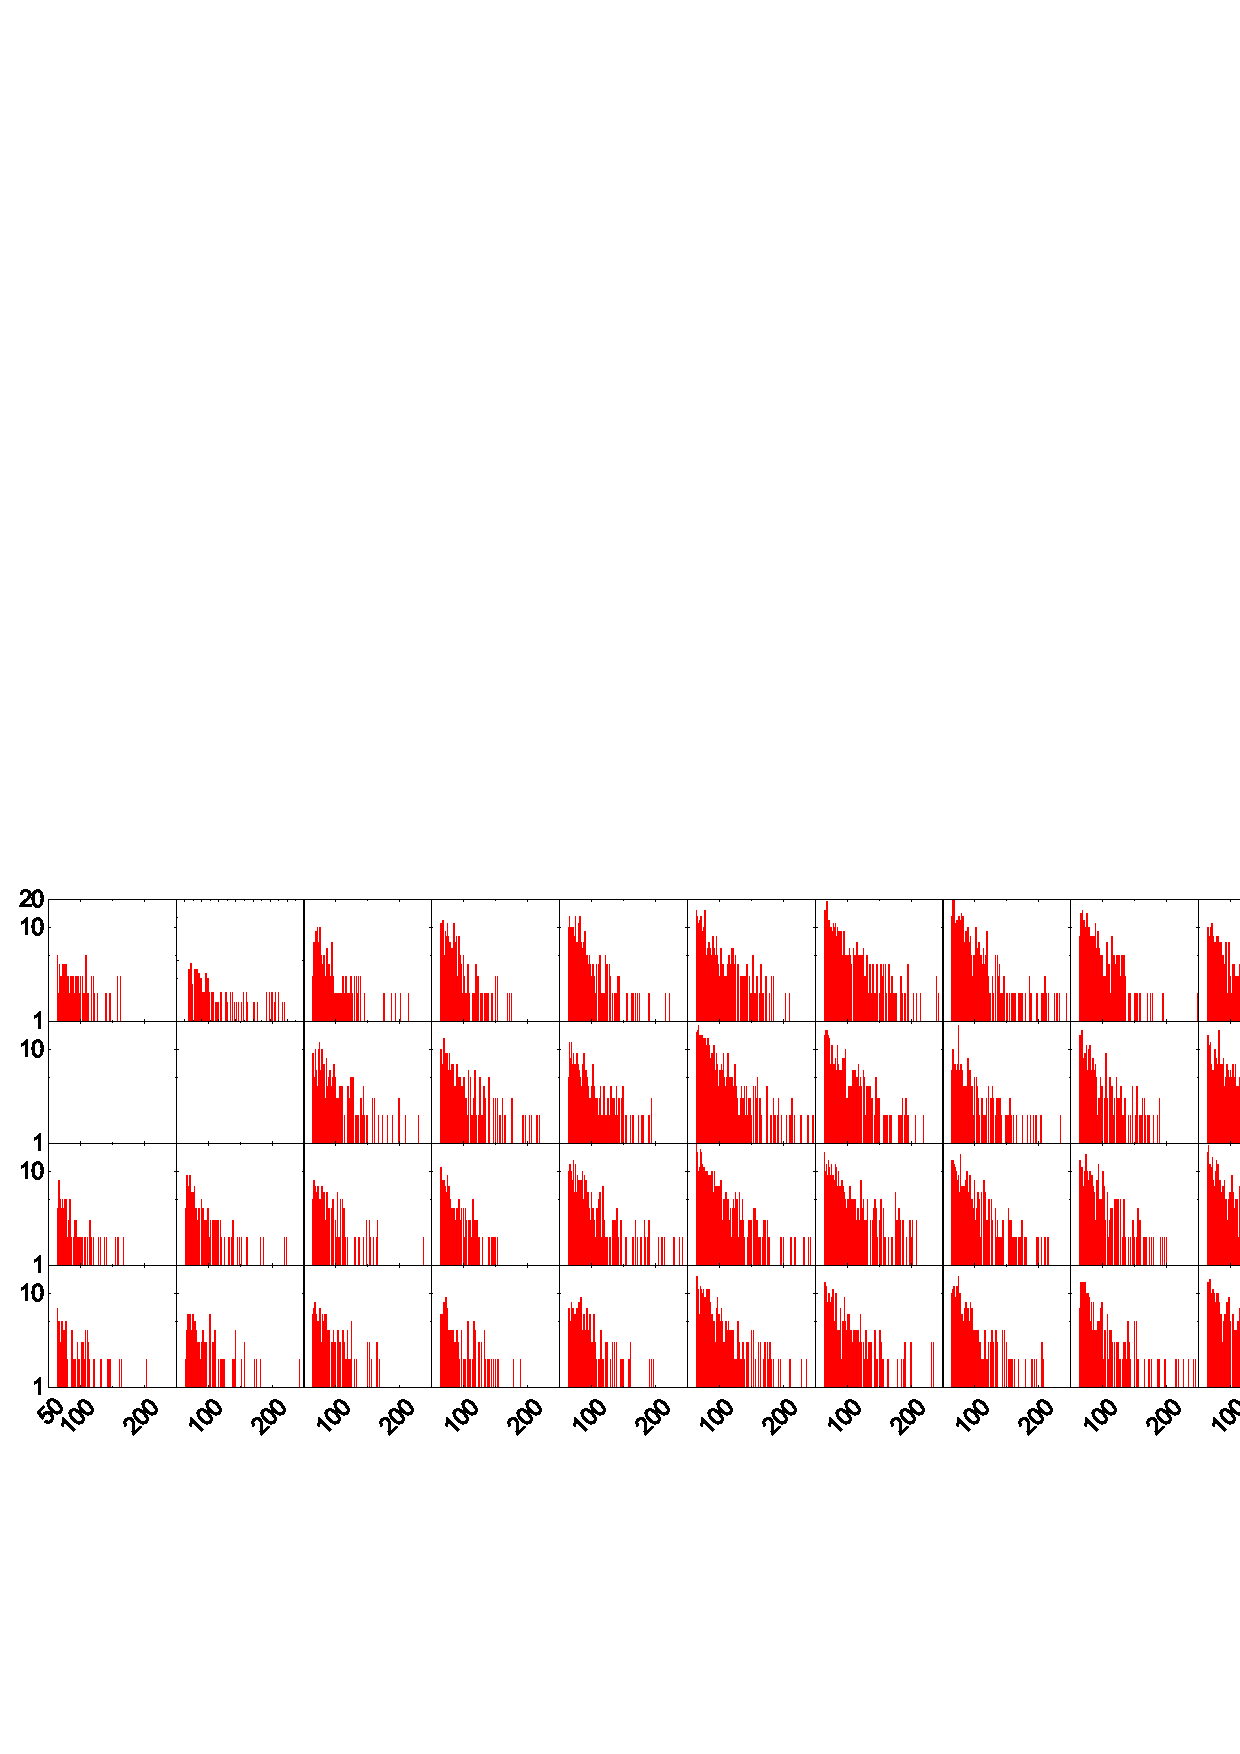
\includegraphics[width=\textwidth]{chapters/figures/flow_burst_size_48_spots.jpg}
\caption{\label{fig:flow_burst_size_48_spots}
Burst size histograms of all photons streams for each spot in the \ac{HT-smFRET} microfluidic experiment discussed in Section~\ref{sec:smFRET_microfluidics}. 
Analysis parameters: \ac{APBS}, $m = 10$, $r_m \geq 80~kHz$,
$\overline{F} \geq 64$. 
Spot 1 is at the top left, spot 12 at the top right. 
Spot 13 and 14 are missing from this series,
due to a malfunction of two SPADs in the donor SPAD array. 
The better illumination of the center spots translates into larger burst statistics.
Details of the analysis can be found in \texttt{ALiX Notebook, Flow, \ac{APBS}, m= 10, Rmin = 80 kHz, Smin = 64.rtf} and associated files in the Figshare repository~\cite{figshare_repo_2019}. 
Figure reprinted from Segal, \textit{et al.}~\cite{segal_methods_2019}.
}
\end{figure}

When the characteristics of different spots are comparable, it is reasonable to combine this data into a unified histogram. 
This approach is illustrated in Fig.~\ref{fig:pooled_burst_size_distributions}, facilitating comparisons between datasets acquired under identical conditions or to assess the impact of various burst search parameters on the burst size distribution.

\begin{figure}
\centering\includegraphics[width=0.7\textwidth]{chapters/figures/pooled_burst_size_distributions.jpg}
\caption{\label{fig:pooled_burst_size_distributions}
Pooled burst size histograms corresponding to the two datasets discussed in section \ref{sec:smFRET_microfluidics}. 
The diffusion only (no flow or \enquote{NF}) dataset, recorded with lower excitation powers (by a factor $\sim1.6$), was analyzed with a lower rate threshold ($r_m \geq 50~kHz$) for burst search and a lower burst size threshold ($\overline{F} \geq 40$, black)
for burst selection, than the dataset recorded with flow (F, red), for which $r_m \geq 80~kHz = 50 \times 1.6, \overline{F} \geq 64 = 40 \times 1.6$, in order to obtain comparable number of bursts for analysis.
For comparison, burst size distributions obtained when using the larger rate threshold for the no flow sample ($r_m \geq 80~kHz$,  NF, gray), or the lower burst size threshold for the sample with flow ($\overline{F} \geq 40$, F, orange) are represented as dashed curves. The red curve corresponds to the sum of all histograms in
Figure~\ref{fig:flow_burst_size_48_spots}.
The higher excitation powers used in the flow measurement more than compensate for the shorter transit time of molecules and more stringent burst search and selection criteria, as can be seen from the larger number and larger sizes of the collected bursts.
Details of the analysis can be found in the different notebooks: \texttt{ALiX Notebook, XX, \ac{APBS}, m = 10, Rmin = YY kHz, Smin = ZZ.rtf} where XX = Flow or No Flow, YY = 50 or 80, ZZ = 40 or 64, and associated files in the Figshare repository~\cite{figshare_repo_2019}. 
Figure reprinted from Segal, \textit{et al.}~\cite{segal_methods_2019}.
}
\end{figure}

\subsection{Burst Duration}
\label{sec:burst_duration_apdx}

Burst duration, as discussed earlier in the context of burst search, is a valuable parameter for a rapid assessment of potential differences in spot sizes or alignment. 
When observing the same sample across all spots, any expected scaling, assuming the spots are similar, should primarily manifest as differences in the number of bursts.
This could occur, for instance, if the excitation power is not uniform across the pattern. 
In such cases, the overall shape of the duration histograms should remain nearly identical, provided that an appropriate burst search using a constant threshold is performed~\cite{ingargiola_PLOS1_2016}. 
If the burst duration histograms exhibit dissimilarity, it is important to investigate potential sources of non-uniformities.

However, it is important to note that the burst duration distribution is a complex function for which no current analytical model exists. 
As discussed previously~\cite{ingargiola_PLOS1_2016}, a practical way to represent these intricate distributions is by using a modified semi-logarithmic histogram introduced by Sigworth and Sine~\cite{sigworth_BJ_1987}. 
This approach was originally developed to study sums of exponentials and offers the advantage of easily identifying the relevant time scale. 
In this \enquote{S\&S} representation, data is binned logarithmically without normalization to account for the variable widths of the bins, and the square root of each bin content is displayed. 
An example of burst duration histograms obtained in the microfluidic \ac{HT-smFRET} measurement discussed in Section~\ref{sec:smFRET_microfluidics} is presented in Fig.~\ref{fig:flow_burst_duration_48_spots}.

\begin{figure}
\centering
\includegraphics[width=\textwidth]{chapters/figures/flow_burst_duration_48_spots.jpg}
\caption{\label{fig:flow_burst_duration_48_spots}
Burst duration histograms in seconds for each spot in the \ac{smFRET} in flow experiment discussed
in Section~\ref{sec:smFRET_microfluidics}. 
Analysis parameters: \ac{APBS}, $m = 10$, $r_m \geq 80~kHz$, $\overline{F} \geq 64$. 
Spot 1 is at the top left, spot 12 at the top right. Spot 13 and 14 are missing from this series, due to a malfunction of two SPADs in the donor SPAD array. 
The better illumination of the center spots translates into larger burst statistics.
Details of the analysis can be found in the notebook \texttt{ALiX Notebook, Flow, \ac{APBS}, m = 10, Rmin = 80 kHz, Smin = 64.rtf}  and associated files in the Figshare repository \cite{figshare_repo_2019}.
Figure reprinted from Segal, \textit{et al.}~\cite{segal_methods_2019}
}
\end{figure}

Similarly to burst sizes, if the characteristics of the spots are similar, it is reasonable to combine this data into a single histogram. 
This approach, demonstrated in Fig.~\ref{fig:pooled_burst_duration}, allows for straightforward comparisons with data acquired under the same conditions.

\begin{figure}
\centering\includegraphics[width=0.7\textwidth]{chapters/figures/pooled_burst_duration.jpg}
\caption{\label{fig:pooled_burst_duration}
Pooled burst duration S \& S histograms corresponding to the two datasets discussed
in section \ref{sec:smFRET_microfluidics}. 
The diffusion only (no flow or NF) dataset, recorded with lower excitation powers (by a factor $\sim1.6$), was analyzed with a lower rate threshold ($r_m \geq 50~kHz$) for burst search and a lower burst size threshold ($\overline{F} \geq 40$, black) for burst selection, than the dataset recorded with flow (F, red), for which $r_m \geq 80~kHz = 50 \times 1.6, \overline{F} \geq 64 = 40 \times 1.6$, in order to obtain comparable number of bursts for analysis.
For comparison, burst durations obtained when using the larger rate threshold for the no flow sample  ($r_m \geq 80~kHz$, NF, gray), or the lower burst size threshold for the sample with flow ($\overline{F} \geq 40$, F, orange) are represented as well. 
The red curve corresponds to the sum of all histograms in Figure~\ref{fig:flow_burst_duration_48_spots}.
The different burst search and selection criteria for each experiment result in different burst duration distributions, illustrating the challenges associated with this type of analysis.
Details of the analysis can be found in the different notebooks: \texttt{ALiX Notebook, XX, \ac{APBS}, m = 10, Rmin = YY kHz, Smin = ZZ.rtf} where XX = Flow or No Flow, YY = 50 or 80, ZZ = 40 or 64, and associated files in the Figshare repository~\cite{figshare_repo_2019}).
Figure reprinted from Segal, \textit{et al.}~\cite{segal_methods_2019}
}
\end{figure}

\subsection{Peak Burst Count Rate}
\label{sec:peak_count_rate_apdx}

The characteristics of bursts, such as those discussed earlier, may be modeled by probability density distributions due to the diffusion of single molecules within the confocal excitation volume. 
In some cases, these distributions can be theoretically modeled, and under favorable conditions, they approach exponential behavior~\cite{gopich_JCP_2006}. 
However, the choice of burst search parameters, including the selection of the photon stream, the value of $m$, the use of fixed or adaptive thresholds, and the application of burst fusion, can impact the observed burst statistics. 
For instance, applying a higher threshold to a burst that starts and ends with low count rates will result in a smaller burst size with a shorter burst duration.

In contrast, the peak count rate within a burst, which represents the maximum photon detection rate using a specific number of photons, is typically determined within the burst itself and is not influenced by burst truncation at its edges.

Hence, while quantities like burst size are intricately linked to the precise trajectory of a molecule through the excitation \ac{PSF}, the peak count rate primarily reflects how closely the molecule's trajectory approached the excitation peak within the spot. 
Therefore, plotting this parameter with a histogram for all bursts provides more direct information about the peak excitation intensity in each spot, which is important for comparing different spots in a multispot setup.

The peak count rate, as defined in the Supporting Information of the FRETBursts publication~\cite{ingargiola_PLOS1_2016}, is:

\begin{equation}
\label{eqn:peak_count_rate}
r^{Y}_{X_{max}} = max(r_m(t_i))
\end{equation}

\noindent
where the $t_i$'s are timestamps within a burst and $r_m(t_i)$ 
is defined by Eqn.~\ref{eqn:local_rate}.

The definition provided in Eqn.~\ref{eqn:peak_count_rate} relies solely on the timestamps $t_i$ within a burst and the rate function $r_m(t_i)$ defined by Eqn.~\ref{eqn:local_rate}. 
However, it doesn't consider laser alternation or specify which excitation cycle a timestamp corresponds to. 
To include laser alternation, the peak count rate requires modification:

\begin{equation}
\label{eqn:peak_count_rate'}
r'^{Y}_{X_{max}} = max\left(\frac{m-2}{\Delta t^{(m)}_{j}} - (p -1)g\right)
\end{equation}

% \noindent
In this equation, $t_j$ and $t_{j+m-1}$ represent the timestamps marking the start and end of a burst, respectively. 
The parameter $g$ represents the minimum time between two donor excitation cycles, and $p$ signifies the number of alternation periods separating the burst.

As with other burst statistics, the outcome of the analysis of a multispot dataset includes a series of histograms for the burst peak count rate, as shown in Fig.~\ref{fig:flow_burst_peak_r_D_D_48_spots}.

\begin{figure}
\centering
\includegraphics[width=\textwidth]{chapters/figures/flow_burst_peak_r_D_D_48_spots.jpg}
\caption{\label{fig:flow_burst_peak_r_D_D_48_spots}
Burst peak count rate histograms during the D-excitation period and in the donor channel for each spot in the microfludic \ac{HT-smFRET} experiment discussed in Section~\ref{sec:smFRET_microfluidics}.
Analysis parameters: \ac{APBS}, $m = 10$, $r_m \geq 80~kHz$,
$\overline{F} \geq 64$. 
Spot 1 is at the top left, spot 12 at the top right. Spot 13 and 14 are missing from this series, due to a malfunction of two SPADs in the donor SPAD array. 
The better illumination of the center spots translates into larger number of bursts, but also larger peak burst rates.
Details of the analysis can be found in the notebook \texttt{ALiX Notebook, Flow, \ac{APBS}, m = 10, Rmin = 80 kHz, Smin = 64.rtf} and associated files in the Figshare repository \cite{figshare_repo_2019}.
Figure reprinted from Segal, \textit{et al.}~\cite{segal_methods_2019}.
}
\end{figure}

Pooling the burst peak count rates from all spots into a single histogram is useful for comparing different experiments, even if some border spots exhibit fewer and dimmer bursts, as can be seen from an examination of the spot intensity pattern shown in Fig.~\ref{fig:setup}. 
This pooled peak count rates are presented in Fig.~\ref{fig:pooled_burst_peak_r_D_D}.

\begin{figure}
\centering
\includegraphics[width=0.7\textwidth]{chapters/figures/pooled_burst_peak_r_D_D.jpg}
\caption{\label{fig:pooled_burst_peak_r_D_D}
Pooled burst peak count rate histograms during the D-excitation period and in the donor channel corresponding to the two datasets discussed in section \ref{sec:smFRET_microfluidics}.
The diffusion only (no flow or NF) dataset, recorded with lower excitation powers (by a factor $\sim1.6$), was analyzed with a lower rate threshold ($r_m \geq 50~kHz$) for burst search and a lower burst size threshold ($\overline{F} \geq 40$, black) for burst selection, than the dataset recorded with flow (F, red), for which $r_m \geq 80~kHz = 50 \times 1.6, \overline{F} \geq 64 = 40 \times 1.6$, in order to obtain comparable number of bursts for analysis.
For comparison, burst size distributions obtained when using the larger rate threshold for the no flow sample  ($r_m \geq 80~kHz$, NF, gray), or the lower burst size threshold for the sample with flow ($\overline{F} \geq 40$, F, orange) are represented as dashed curves. 
The red curve corresponds to the sum of all histograms in
Figure \ref{fig:flow_burst_peak_r_D_D_48_spots}.
As argued in the text, the asymptotic part of the burst peak count rate distribution is insensitive to the exact burst search and selection parameters used in the analysis, as is clear from the overlap of the exponential tails of the two no flow (NF, black and gray) and the two flow (F, red and orange) curves.
The ratio of the two exponential coefficients (F: 216 kHz and NF: 116 kHz, $F/NF = 1.9$) is approximately equal to the ratio of the donor laser  excitation powers used in the two measurements ($500/300 = 1.7$), as expected.
Details of the analysis can be found in the different notebooks:
\texttt{ALiX Notebook, XX, \ac{APBS}, m = 10, Rmin = YY kHz, Smin = ZZ.rtf} where XX = Flow or No Flow, YY = 50 or 80, ZZ = 40 or 64, and associated files in the Figshare repository~\cite{figshare_repo_2019}.
Figure reprinted from Segal, \textit{et al.}~\cite{segal_methods_2019}.
}
\end{figure}

\section{Fluorescence Correlation Analysis}
\label{sec:fcs_analysis_apdx}

\ac{FCS} can be performed on single or multispot setups to characterize the excitation-detection volumes sampled by the donor and acceptor, determine diffusion coefficients, brightness, and, when sufficient statistics are available, it can be utilized to study short time-scale dynamics~\cite{krichevsky_RPP_2002}. 
In the case of multispot experiments, \ac{FCS} analysis is particularly helpful in detecting otherwise challenging-to-quantify differences in spot characteristics. 
One of the simplest pieces of information that can be readily extracted from this analysis is the diffusion time through the excitation-detection volume, $\tau_D$, which is a useful indication of variations between spots.

In previous studies, we have conducted comparisons of single and multispot setups using FCS analysis~\cite{colyer_BOE_2010,ingargiola_PLOS1_2016, ingargiola_JCP_2018}. 
This analysis can be performed on the same dye, resulting in the \ac{ACF}, or on two different dyes, leading to the \ac{CCF}.
\ac{CCF} analysis can also be performed using a single dye, as in the case of \ac{ACF}, however, these measurements require a optical beamsplitter for detection in two separate channels.
\ac{FCS} analysis is complementary to burst duration and brightness analysis, as it can be used to reveal subtle differences in effective excitation-detection volumes or peak excitation intensities~\cite{ingargiola_PLOS1_2016}.

Quantitative \ac{FCS} analysis can be affected by various experimental artifacts and may require simplifying assumptions that are not always met~\cite{hess_BJ_2002, enderlein_CPB_2004}. 
One significant challenge is that current \ac{SPAD} arrays can exhibit afterpulsing and other effects at short time scales ($< 1 \mu$s), which complicates the routine use of the \ac{ACF} as a tool for analysis using \ac{SPAD} detectors.

\ac{CCF} analysis, in contrast, can alleviate many of these issues. 
In \ac{smFRET} experiments with two detection channels, it is primarily limited to correlating donor and acceptor signals within a spot. 
However, when examining separate spots, there are no such limitations. 
In diffusion experiments, cross-correlating signals from different spots might not provide information on a sample, as the distance between spots is typically on the order of $5~\mu$m, which is too large to extract meaningful diffusion coefficient information. 
If analyzing the capabilities of a \ac{SPAD} array, \ac{CCF} analysis can be used to measure optical crosstalk between pixels within a single detection channel~\cite{ingargiola_PLOS1_2016, ingargiola_NIMA_2018}.

However, as demonstrated in Section~\ref{sec:microfluidics_CCF}, \ac{CCF} analysis between \ac{SPAD}s within a single detection channel can be effectively employed to extract flow velocity as well as the direction of flow~\cite{brinkmeier_AC_1999}. 
Additionally, by analyzing the average \ac{CCF} of all spots, enhanced statistical accuracy can be achieved, as illustrated in Fig.~\ref{fig:flow_analysis}. 

Future iterations of a multispot setup might incorporate two \ac{SPAD} arrays per channel, enabling \ac{CCF} analysis within single spots and channels. 
This advancement would provide access to short timescale dynamics. By appropriately accounting for spot-specific differences and averaging \ac{CCF} curves from multiple spots, the time required to accumulate sufficient statistics for studying short timescale dynamics could be significantly reduced~\cite{felekyan_RSI_2005}.
